\documentclass[letterpaper,12pt]{exam}
\usepackage{csc274videonotes}

\newcommand{\unit}{Unit 01}
\pagestyle{headandfoot}
\firstpageheader{CSC 274 \semester\ \  \unit}{}{Name: $\rule{6cm}{0.15mm}$}
\runningheader{CSC 274 \semester}{\unit}{Page \thepage\ of \numpages}
\firstpagefooter{}{}{}
\runningfooter{}{}{}

\usepackage{draftwatermark}
\SetWatermarkText{CSC 274}
\SetWatermarkScale{.7}
\SetWatermarkColor[rgb]{0.8,0.8,0.8}

\begin{document}

\begin{itemize}
	\item Print out these pages.  If you do not have access to a printer, please contact the instructor.
	\item Handwrite your answers on the pages you print out. Do not type them.
	   \begin{itemize}
		  \item \textbf{I will not accept just the answers written on a sheet of paper.}  
		  \item \textbf{I will not accept typed output.}
	   \end{itemize}
	\item If you have a flatbed scanner, please scan the images into a .pdf file.  
	  \begin{itemize}
         \item PDF files are much better than individual jpg files.
         \item If you don't have a flatbed scanner, please use a "camscanner" app on your phone to produce a single .pdf file for the assignment.
      \end{itemize}

	\item The video notes are intended as \textbf{learning aids} and not grading exercises.
	\item Watch the videos and fill these pages out as you go.
	\item I will only spot check a few questions and look for completeness.  There are only a few ways you can lose points:
	   \begin{itemize}
	     \item Skip a question or give a frivolous answer. 
		 \item Just copy some answer you found on the internet.  Instead, use your own words.
	     \item Cheat.  Don't use another student's answers, although it is fine (and encouraged) if you talk over specific questions with another student.  Just be sure to give your own answer and don't copy another student.  Also, don't use notes from another semester; I can be sneaky.
	   \end{itemize}
	\end{itemize}

If you don't know an answer try to figure it out.  Instead of an answer,
write about what you do understand or why you are confused.  Maybe put a big \textcolor{BrickRed}{\Huge*} or \textcolor{BrickRed}{\Huge?} in the margin next to 
the question.


\section*{Unit 01\_03 --- Videos and Notes} % Unnumbered section

\begin{questions}
\question How are you filling out these notes?
\begin{checkboxes}
\choice I am writing the answers on a sheet of notebook paper which I will turn in (This is a wrong answer.)
\choice I am typing the answers (This is also a wrong answer)
\choice I am hand-writing the notes on printed copies of the .pdf file from the handouts. (This is the correct answer.)
\end{checkboxes}

\question What is the url of the github repository where you can find the notes? 
\vspace{.75cm}

\question In your own words, explain at least two ways you can lose points on these notes. 
\vspace{1.5cm}

\question What are the exams based on?
\begin{checkboxes}
\choice Only these written notes
\choice Only the videos
\choice Only the handouts
\choice Only the homework
\choice The notes, videos, handouts, and homework
\end{checkboxes}

\end{questions}
%%%%%%%%%%%%%%%%%%%%%%%%%%%%%
\section*{Unit 01\_05 --- Overview and History}
\subsection*{Video A}

\begin{questions}
	\question  In your own words, what is the kernel of the operating system? (You may look up kernel on the Internet, but I want you to use your own words.  I almost never want you to just copy something that you find in the notes or online.)
	\vspace{1.5cm}

	\question What is the Interface? 
	\vspace{1.5cm}	

	\question What is the main interface we will be leaning this semester? 
	\vspace{1.5cm}

	\question In what decade was Unix developed?
	\begin{checkboxes}
	\choice 1950s
	\choice 1960s
	\choice 1970s
	\choice 1980s
	\end{checkboxes}

	\question Who was Linus Torvalds? 
	\vspace{1.0cm}

\question  What are at least two tasks performed by the Operating System?
\vspace{1.5cm}

\question List two things from the development of Unix in the 1970s that still influence us today in this course, not counting the development of Unix itself.
\begin{checkboxes}
\choice {\Huge \textcolor{white}{X}} 
\choice {\Huge \textcolor{white}{X}}
\end{checkboxes}

\subsection*{Video B}

\question In your own words, what does "parsimonious" mean? 
\vspace{1.5cm}

\question An old saying is that "Unix is parcimonious." Give an example that illustrates this. 
\vspace{1.5cm}

\question Why did teletype machines create an incentive for the developers of Unix to keep commands and output short. 
\vspace{1.5cm}

\question What is a dumb terminal? Why isn't a dumb terminal considered a computer?
\vspace{1.5cm}

\question What is a shell?
\vspace{1.5cm}

\question What is Bash? 
\vspace{1.5cm}


\question About 10 years ago the announcement was made that the majority of the world's computers now run Linux.  It is still a true statement.  It sounds counter-intuitive because most people run Windows or Mac OS on their desktops and laptops; Linux laptop and desktop users are fairly rare.  Many servers and supercomputers run Linux, however, there is a relatively small number of these compared to desktop units.  So why is it accurate to say that more computers run Linux than any other operating system? (Hint: The answer is probably in your pocket, unless you have an iPhone.) 
\vspace{1.5cm}
%%%%%%%%%%%%%%%%%%%%%%%%%%%%%
\section*{Unit 01\_10 --- woz}

\question In the CSMP server room we generally name the servers for people important to the history of computers.  Where did the name "woz" come from?  (This is an example of a question that isn't in the video.  You might or might need to search the Internet for an answer.)
\begin{figure}[h]
	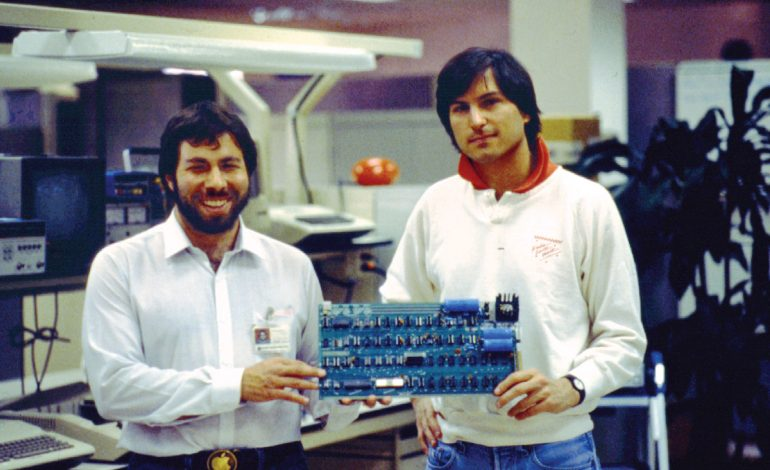
\includegraphics[width=6cm,right]{s_and_w}
\end{figure}

\question What operating system do you plan to use on your personal laptop or desktop this semester? (Not including the woz server)
\begin{checkboxes}
\choice Windows 10
\choice Windows, but not 10
\choice Mac OS
\choice Linux
\end{checkboxes}

\begin{samepage}
\question How do you expect to connect to Woz? 
\begin{checkboxes}
\choice putty
\choice ssh
\choice other (Please specify):
\end{checkboxes}
\end{samepage}

Note:  There are no notes on the optional videos, but you should watch the video corresponding to the method you expect to use to connect.

Please try to connect before class starts.  I will send out an email saying what the password is.  It may also be in the optional videos.

\question  Tux the penguin is the Mascot of Linux.  There is a picture of Tux at the end of each set of notes.  What is the significance of the gnu sitting behind Tux in the picture below?
\vspace{1.5cm}

\end{questions}
\begin{figure}[b]\label{end}
	\center
	
\includegraphics[width=1in]{tux}
	{\center{Tux with a gnu}}
\end{figure}
\end{document}